\begin{frame}{Assignment Problem}
\begin{figure}
    \centering
    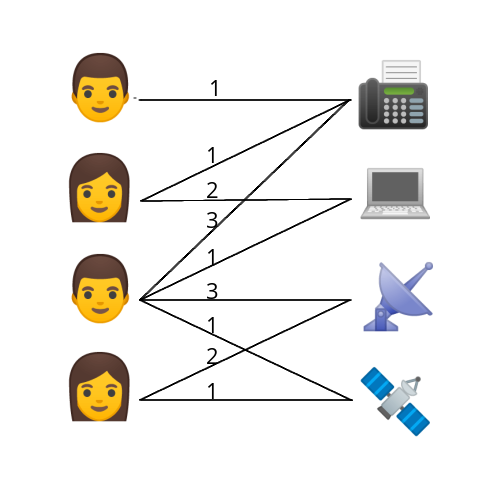
\includegraphics[height=5cm]{img/introduction/assignment.png}
\end{figure}
\end{frame}

\begin{frame}{Definitions}
        \begin{itemize}[<+->]
    \item Matching
    \item Perfect Matching
    \item \textbf{Bipartite} Matching
    \item Maximum Matching
    \end{itemize}
  
  %add different figure for perfect matching and bipartite matching  
\only<1>{
\begin{figure}
\begin{subfigure}{.5\textwidth}
\centering

\includegraphics[width=.4\linewidth]{img/introduction/graph01.eps}
\end{subfigure}%
\begin{subfigure}{.5\textwidth}
\centering
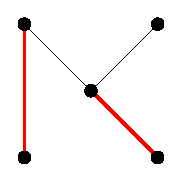
\includegraphics[width=.4\linewidth]{img/introduction/graph02.eps}
\end{subfigure}
\end{figure}
}
\only<2>
{
\begin{figure}
    \centering
    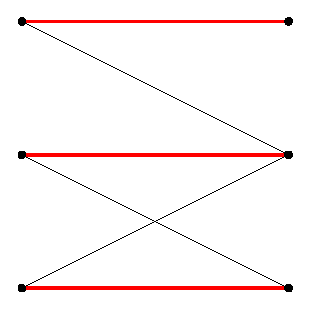
\includegraphics[width=0.3\linewidth]{img/introduction/perfectmatching.eps}
\end{figure}
}
\only<3>{
\begin{figure}
\begin{subfigure}{.5\textwidth}
\centering
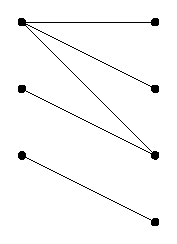
\includegraphics[width=.4\linewidth]{img/introduction/bipar.eps}
\end{subfigure}%
\begin{subfigure}{.5\textwidth}
\centering
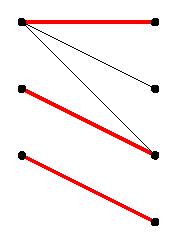
\includegraphics[width=.4\linewidth]{img/introduction/biparmatch.eps}
\end{subfigure}
\end{figure}
}
\only<4>{
\begin{figure}
\begin{subfigure}{.5\textwidth}
\centering
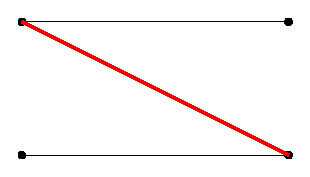
\includegraphics[width=.4\linewidth]{img/introduction/maximalmatch.eps}
\end{subfigure}%
\begin{subfigure}{.5\textwidth}
\centering
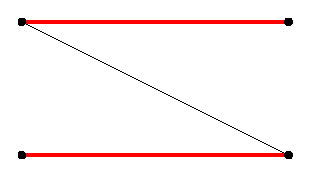
\includegraphics[width=.4\linewidth]{img/introduction/maximummatching.eps}
\end{subfigure}
\end{figure}
}
    
\begin{block}{Definition}
    \only<1>{A set of non overlapping edges.}
    \only<2>{Matching of size $\frac{|V\left(G\right)|}{2}$}
    \only<3>{Matching of the maximum size.}
    \only<4>{Matching on a bipartite graph.}
\end{block} 
\end{frame}